\documentclass[../main.tex]{subfiles}

\usepackage{listings}
\usepackage{setspace}

\begin{document}
\newpage

\chapter{The Finite Element Method }

\subsection{A NONTECHNICAL OVERVIEW OF THE FINITE ELEMENT 
METHOD}

The Finite Element Method (FEM) is actually a large collection of numerical methods for solving PDEs. It was first devised as a numerical tool by mathematician Richard Courant
\footnote{Richard Courant was an exceptionally influential mathematician. He grew up in Germany and had a rather difficult childhood, having to work to help support his family while going to school. He eventually entered the Univerisity of Breslau (now Wroclaw, Poland) as an undergraduate and was lured to major in mathematics by the exciting lectures in his classes. He went on to Göttingen for his graduate studies where he worked with Hubert and later became a professor there. His education was interrupted by military service for Germany in WWI, where he developed an effective electronic communications system that was implemented for the troops. Despite the important contributions he was making to the University of Göttingen, not to mention his important military service to his country, when the Nazis came to power in the early 1930s, he was forced to resign his professorship. The Nazis had decreed that any "non-Aryan" civil servant was to be terminated and having one Jewish grandparent was sufficient to make someone "non-Aryan." There was supposed to be an exemption for individuals who gave Germany military service in WWI, but despite ardent efforts on the part of the university to keep him, Courant was still "retired." He subsequently accepted an offer at New York University. The transition was very difficult for him. Coming from a world-renowned institute and having been surrounded by top-notch mathematicians, when he got to NYU, he found his colleagues to be very weak and the students likewise poor. He made use, however, of his extensive contacts and was able to hire a large group of strong new faculty. Today, NYU's mathematics department, also known as the \textit{Courant Institute}, is considered by many as the premiere applied mathematics institute in the world.}in a 1943 paper on torsion problems [Cou-43], and is based on analogous techniques and principles to those developed in the early twentieth century for one-dimensional boundary value problems, as were presented in Section 10.5. The method was extensively elaborated on during the 1950s and 1960s by engineers as a practical approach for solving various PDEs in structural engineering. In the 1960s and 1970s, mathematicians worked to give the method a solid theoretical basis and extended it as a tool for solving many different PDE problems. Active research on this method continues today and it has become the most commonly used numerical method for partial differential equations. As a very pertinent example, in MATLAB's PDE Toolbox, all of the programs for solving PDEs use FEMs. Writing even somewhat general programs for FEMs is a very complicated task. Our goal in this chapter will be to explain the method and to write some programs to implement it in several specific instances. This should be sufficient for readers needing to delve deeper into FEMs to be able to extend the programs into more general ones. MATLAB's PDE Symbolic Toolbox programs are open to its users to read and modify. So, in principle, after reading this chapter, readers could modify some of the FEM programs in MATLAB's toolbox to suit their exact needs (if notalready met). 

\begin{wrapfigure}{l}{0.2\textwidth}
    \centering
    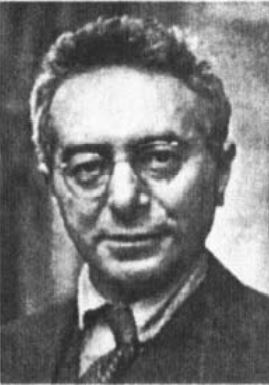
\includegraphics[width=0.2\textwidth]{ch13_1}
   \caption{\textsf{Richard Courant (1888-1972), German mathematician }}
   \label{fig:ch13_2}
\end{wrapfigure}

The FEM methods basically split up the domain of the problem into small pieces, called \textbf{elements}, that have simple structure. There are many different ways to perform such decompositions and the geometry certainly changes with the dimension of the space. A common approach for two-dimensional domains is to \textbf{triangulate} the domain into small triangles. The \textbf{triangulation} must be done in such a way that whenever two triangles touch, they will have either an entire common edge (and thus two common vertices) or just a common vertex. The reason for this is that the FEM approximate solution for the PDE will be made up of separate "pieces" on the various elements and they need to connect up (interpolate) together in a neat fashion. When a domain has a curved boundary, the sizes of the triangles can be made small enough so that the triangulation approximates the domain reasonably well. An example of such a triangulation is shown in Figure 13.2. In three dimensions, tetrahedra (pyramids) are commonly used; but the process is still known as triangulation.
\newpage
\begin{figure}[H]
	\centering
	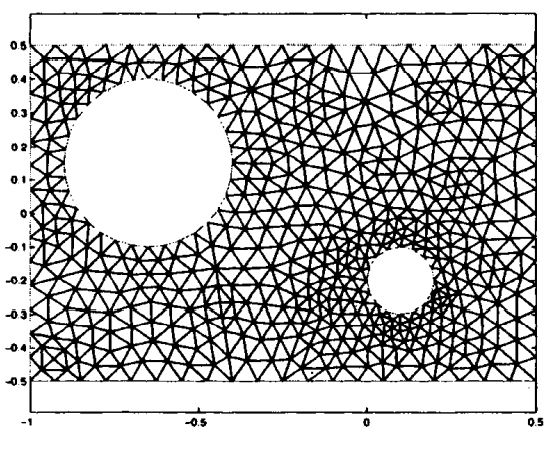
\includegraphics[width=0.6\linewidth]{ch13_2}
	\caption{\textsf{A triangulation of a planar domain consisting of a rectangle with two circles deleted. The circular boundary portions are thus approximated by polygons (as shown). This triangulation was created using MATLAB's PDE Toolbox. }}
	\label{pfig:ch13_2}
\end{figure}
Even in two dimensions, of course, there are numerous ways to perform such a triangulation. We point out some important features of the triangulation in Figure 13.2. First, notice that the triangles in the mesh all seem to be roughly the same size. This uniformity is not necessary, but for a general problem on a given domain it is usually the best generic triangulation scheme. Another important property is that none of the sidelengths of any triangle in the mesh is much shorter than the other two sides of the same triangle. Another way to describe this property is that the area of the inscribed circle of any of thesetriangles is not much smaller than the area of the triangle. This feature is essential in order that the finite element method be stable. 
\\

Just writing a good program to create such generic triangulations is already an arduous task. It must be thought out how the geometry of the original domain should be inputted (as a matrix) and then the triangles must be created and stored, usually by their vertices. Additionally, the vertices of the triangulation will need to be numbered and it will be helpful for the numbering to be done in such a way that the numbers of the three vertices of any triangle are reasonably close. 
\\

Like finite difference methods, finite element methods will discretize the PDE 
into a linear system. The nature of the discretization, however, is very different 
for FEMs. Mathematically, the PDE is first converted to a so-called \textbf{variational 
problem}. This is usually done in one of two ways: the \textbf{Rayleigh-Ritz method}, 
where the solution of the PDE is recast as the solution of a certain minimization 
problem among a large class of functions, or the Galerkin method, where the 
solution is recast as a certain unique representing function. Although different in 
philosophy, the two approaches often turn out to be equivalent. With either 
method, the approximate solution is found by restricting attention to a certain 
finite-dimensional space of so-called \textbf{admissible functions} determined by \textbf{basis 
functions} corresponding to each of the elements. Even with the type of elements 
being specified, there are numerous choices for the basis functions. The simplest 
choice would be constant functions, but these do not blend together well. The next 
simplest choice would be to have linear functions on each element. For two dimensional domains with triangulations, this type of basis function turns out to be 
quite effective. Over each element, the graph of such a basis function will be the 
triangular portion of a plane (sitting over the two-dimensional triangle). Since 
three points determine a plane, these basis functions will be flexible enough to 
accommodate specifying values at the three vertices of their triangle, and mesh 
triangles that have common vertices or edges will have their graphs coinciding at 
common points. The resulting approximating functions will thus be continuous 
over the original domain, but in general will not be differentiable at common 
edges or vertices of different triangles. More complicated spline-type basis 
functions can be used to overcome this differentiability problem, but, of course, 
the limited benefits of using such more complicated basis functions would have to 
be weighed against the resulting increase in technical difficulties. For most 
applications on two-dimensional domains with triangular elements, such linear 
basis functions are sufficient and most commonly used. MATLAB's PDE Toolbox, for example, uses such basis functions.
\footnote{The programs in MATLAB's PDE toolbox are designed only to handle PDEs with two space 
variables, and so, for example, they cannot solve three-dimensional elliptic problems such as steadystate heat distributions and structure of materials. The programs can, however, accommodate a time  in hyperbolic or parabolic equations. The reason for this is that FEMs for parabolic and hyperbolic problems invoke finite difference schemes for the time derivatives and thus can accommodate two space variables in addition to the time variable. }
\\
Focusing only on (linear combinations of) the basis functions, the FEM will solve 
a linear system to determine the best candidate to solve the variational problem 
(Rayleigh-Ritz or Galerkin) and this will be the approximation to the actual solution. This approximation turns out to be simply theprojection of the actual solution onto the finite-dimensional space of admissible functions or, informally, the best admissible function for solving the variational problem. Figure 13.3 shows the FEM solution for the following PDE problem on the domain $\Omega$ of 
Figure 13.2: 

\begin{equation}
\begin{cases}
\bigtriangleup u=0~~on~~\Omega, ~~~~u=u(x,y)\\
		\partial u/\partial n=0 ~~$on outer rectangle$\\
		u=40, ~~ $on small circle$, u = 500 , $on large circle$
\end{cases}
\end{equation}

\begin{figure}[H]
	\centering
	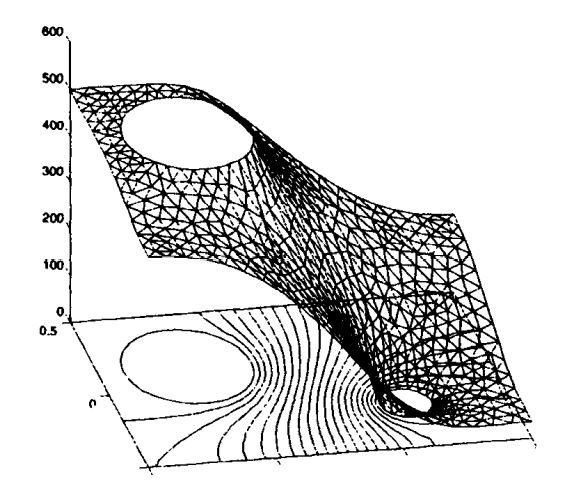
\includegraphics[width=0.6\linewidth]{ch13_3}
	\caption{\textsf{A FEM solution of the steady-state heat problem (1) on the domain and triangulation as pictured in Figure 13.2. Contour lines have been added. This solution was created using MATLAB's PDE Toolbox.}}
	\label{pfig:ch13_3}
\end{figure}

The problem can be thought of as the steady-state heat distribution on the rectangular region $\Omega$ (from the Laplace equation $\bigtriangleup u = 0$). The first boundary condition on the edge of the outer rectangle: $\partial u /\partial n=0$, is a Neumann boundary condition (n denotes the unit outward normal vector for the domain), stating that heat does not flow out of or into the rectangle (i.e., the boundary is insulated). The two constant temperatures on the interior circular boundaries are Dirichlet boundary conditions specifying certain temperatures that are fixed on each. The problem may be thought of as a basic version of the cooling of a nuclear reactor within some enclosed region (the rectangle); the large very hot circle denoting the reactor and the small circle denoting the cooling source (usuallya stream of fresh water). 
\\

In the triangulation process, it is not always efficient to make the triangles be all of essentially the same size. Indeed, at places where the solution varies drastically, smaller triangles should be used and in areas of small variation larger ones can be and should be used. More triangles entail more work so we should use very small ones only where they are needed. Of course, not knowing the solution ahead of time can make it difficult to predict where the solution will be varying wildly. Sharp corners or curves in the domain, as well as areas where the coefficients of the PDE (if variable) rapidly change, are usually problem areas. There are more sophisticated so-called \textbf{adaptive methods} of the FEM that iteratively take into account all available information so as to refine the elements accordingly in a way that aims to reach the best possible accuracy with specified constraints (such as operating time, number of triangles, etc.). Figure 13.4 shows such an adaptive triangularon for the boundary value problem (1). Triangulation of domains is an art!

\begin{figure}[H]
	\centering
	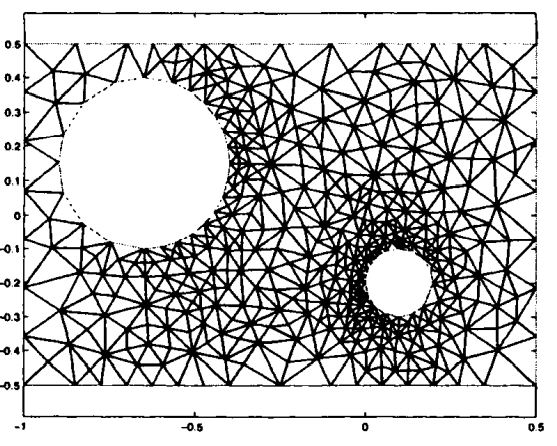
\includegraphics[width=0.6\linewidth]{ch13_4}
	\caption{\textsf{A triangularon of the planar domain of Figure 13.2 that was obtained using an adaptive FEM to solve the steady-state heat problem (1). Compare with the triangularon of Figure 13.2 and, in particular, notice how the triangles closer to the boundaries of the circles (facing inward) are much smaller than the farther away triangles. This triangularon was created using MATLAB's PDE Toolbox. .}}
	\label{pfig:ch13_4}
\end{figure}

An outline for the rest of this chapter is as follows: We will be focusing on linear 
elliptic boundary value problems on planar domains. Our FEM will use piecewise 
linear basis functions on triangulations of the domains. Section 13.2 will 
introduce some practical techniques for producing effective triangulations of 
planar domains and explain how to construct and manipulate basis functions. 
Section 13.3 will explain the complete program of using a FEM to solve quite 
general boundary value problems on arbitrary planar domains and boundary 
conditions. The most time-consuming step of the FEM is the construction of the 
linear system whose solution will give the values of the approximate solution. 
This process, known as "the assembly process," is broken up into an element-by-element computation involving the calculation of certain double integrals and 
(depending on the boundary data) line integrals. We will demonstrate with 
examples that it is not efficient to use MATLAB's integration tools in the 
assembly process. Indeed, if the elements are sufficiently small (depending on the coefficients of the problem), it turns out to be perfectly adequate to use some 
simple numerical quadrature formulas (for triangles and line segments). This will 
allow us to attain essentially the same accuracy as with the more elaborate 
integrators but at a very small fraction of the time. In numerical differential 
equations, much can be learned from experimentation, and this chapter provides 
numerous opportunities in this area. The committed reader can gain a great deal 
by exploring some of the more advanced topics that are introduced in the 
exercises. 

\subsection{TWO-DIMENSIONAL MESH GENERATION AND BASIS 
FUNCTIONS}

Theoretically, the finite element method for two-dimensional problems shares 
many common threads with the one-dimensional Rayleigh-Ritz methods 
introduced in Section 10.5. It would behoove the reader to glance over that 
section periodically as he or she proceeds to work through this and the next 
section. The major practical difference is in the geometry of the two-dimensional 
elements and basis functions versus the very simple one-dimensional elements. 
We will restrict our focus in the text of this chapter to triangular elements and 
piecewise linear basis ftinctions, although some of the exercises will delve into 
other sorts of elements and basis functions. In this section we show how 
triangulations can be created and give some convenient methods for constructing, 
storing, and manipulating corresponding basis functions. 
\\
The two main advantages of the FEM over finite difference methods are its ease in 
dealing with more complicated domains than simply rectangular ones, and its 
flexibility in dealing with many sorts of boundary conditions. To illustrate 
construction of the basis functions, we use the simple triangulation of the 
hexagonal domain shown in Figure 13.5.

\begin{figure}[H]
	\centering
	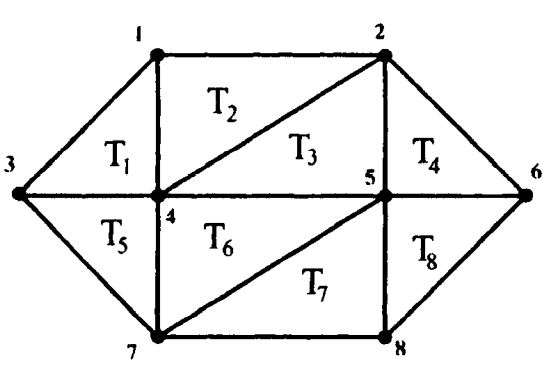
\includegraphics[width=0.5\linewidth]{ch13_5}
	\caption{\textsf{A simple triangulation of a hexagonal domain. The eight nodes are labeled in red and the eight triangles are also labeled. The ordering is somewhat arbitrary. It is just a coincidence that the number of nodes coincides with the number of triangles. At this point we left out x- and y-coordinates so as to emphasize the element numbering.}}
	\label{pfig:ch13_5}
\end{figure}

The \textbf{nodes} in a triangulation are simply the vertices of the triangles. As in the one-dimensional method, each node gives rise to a basis function that takes on the value 1 at its corresponding node and zero at all other nodes. Piecewise linear functions work well here since a linear function is completely determined on a 
triangle once its values are specified on the three vertices. Furthermore, two linear 
functions so determined on triangles that share an edge will agree on the common 
edge. The resulting basis function will be the unique piecewise linear function on 
the hexagon having the property that it is linear on each element and takes on the 
value 1 at its associated node and 0 at all other nodes. In this context the basis 
functions are sometimes known as \textbf{pyramid functions}. The pyramid function for 
the node $\#4$ of Figure 13.5 is illustrated in Figure 13.6. 

\begin{figure}[H]
	\centering
	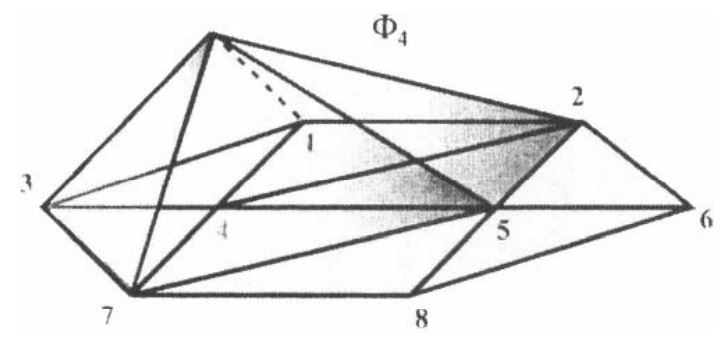
\includegraphics[width=0.5\linewidth]{ch13_6}
	\caption{\textsf{A graph of the piecewise linear basis or pyramid function $\Phi_4 =\Phi_4 (x,y)$ for node $\#4$ in the triangularon of the hexagonal domain of Figure 13.5. The function takes on the value 1 at node $\#4$, zero at all other nodes, and is linear on each triangle. Thus, on the unshaded triangles, the pyramid function is identically zero. 
}}
	\label{pfig:ch13_6}
\end{figure}

To get formulas for the pyramid functions, we need to introduce coordinates. For  purpose of an example, we assign coordinates as follows: node $\#3$ will be put at the origin $(0,0)$, node $\#4$ will have coordinates $(1,0$), and the coordinates of nodes $\#1$ and $\#7$ are $(1,1)$, and $(1,-1)$, respectively. The corresponding  of nodes $\#2$, $\#5$, and $\#8$ are obtained by adding 3/2 to the first coordinates of the last three, and node $\#6$ has coordinates $(7/2,0)$. Knowing these coordinates, all of the information of the triangulation can be represented by the following two matrices, Abodes) and 71(riangles): 
$$
N~=~\begin{bmatrix} 
		  1&1\\
		  2.5&1\\
		  0&0\\
		  1&0\\
		  2.5&0\\
		  3.5&0\\
		  1&-1\\
		  2.5&-1\\
\end{bmatrix},
~~~~
T~=~\begin{bmatrix} 
		  1&3&4\\
		  1&2&4\\
		  2&4&5\\
		  2&5&6\\
		  3&4&7\\
		  4&5&7\\
		  5&7&8\\
		  5&6&8\\
\end{bmatrix}
$$

The eight rows of $N$ give the coordinates of the corresponding numbered nodes, the first column entry gives the x-coordinates, and the second column entry the y-coordinates. The eight rows of $T$ give the node numbers of the corresponding numbered triangles, in order (see Figure 13.5). Such matrices will be needed in writing programs for the FEM.
\\
\\
\subsubsection{EXAMPLE 13.1:}Write down a formula for the basis function $\Phi_4 =\Phi_4 (x,y)$ shown in Figure 13.6. 
\\
\\
SOLUTION: From its piecewise linearity, on each of the eight triangles $T_t (1\leqslant \mathfrak{l} \leqslant 8)\Phi_4(x,y), $ will be a linear function and so can be written as

\begin{equation}
\Phi_4(x,y)=a_t^4x+b_t^4y+c_t^4=a_tx+b_ty+c_t,~~(x,y) \in T_t,
\end{equation}
where $a_t^4x+b_t^4y+c_t^4=c_t$ are real constants to be determined.
\footnote{The superscipts, although technically necessary, can be omitted in this example since there is only one 
basis function under consideration. }
We now fix an index $\mathfrak{l}$ and let the three nodes of $T_t$ be denoted by $(x_r,y_r), (x_s,y_s)$> and $(x_t>y_t)$ where $t = 4$. The graph of such a linear function $z = \Phi_4(x,y)$ is a plane in three-dimensional space determined by the three nodal values $\Phi_4(x_r ,y_r ) = 0, \Phi_4(x_s,s_s) = 0$, and $\Phi_4(x_t,y_t) = 1$. These nodal equations may be expressed as the following linear system: 

\begin{equation}
	\begin{cases}
		a_t x_r+b_t y_r+c_t=0\\
		a_t x_s+b_t y_s+c_t=0\\
		a_t x_t+b_t y_t+c_t=0
	\end{cases}
\end{equation}
Putting (3) in matrix notation gives:


\begin{equation}
MA~=~Z, ~~where~~M=
	\begin{bmatrix} 
		  x_r&y_r&1\\
		  x_s&y_s&1\\
		  x_t&y_t&1\\	 
	\end{bmatrix},~~
	A~=~
	\begin{bmatrix} 
		  a_r\\
		  b_s\\
		  c_t\\	 
	\end{bmatrix},~~ and~~Z~=~
	\begin{bmatrix} 
		  0\\
		  0\\
		  1\\	 
	\end{bmatrix}
\end{equation}
Geometrically, since three noncollinear points determine a unique plane, it follows that the linear system (3)/(4) will have a unique solution as long as the three nodes are not collinear. This is certainly the case for any triangulation. We mention one further important point that the system will be well conditioned provided that the area of the triangle $T_t$ is not much greater than that of the inscribed circle. This is a quantitive way of saying that the three nodes of Tt should not be close to being collinear (convince yourself of this!). This can be analytically verified using the following explicit formulas for the determinant of $M$ and $M^{-1}$ : 

\begin{equation}
	|det(M)|=2 \cdot area(T_t),
\end{equation}

\begin{equation}
	M^{-1}=\dfrac{1}{det(M)}
	\begin{bmatrix} 
		  (y_s-y_t) & (y_t-y_r) & (y_r-y_s)\\
		  (x_t-x_s) & (x_r-x_t) & (x_s-x_r)\\
		  (x_s y_t -x_t y_s) & (x_t y_r -x_t y_t & (x_r y_s -x_s y_r\\	 
	\end{bmatrix}
\end{equation}
For a proof of the interesting equation (5), the reader is referred to Exercise 22. 
 (5), equation (6) can be proved by a direct (albeit tedious) verification. Equations (5) and (6) plainly show that the matrix is well conditioned as long as the triangle is not too long and thin. Apart from this, the explicit formula (6) is useful to build into large-scale FEM programs where such matrices need to be inverted large numbers of times in constructing the basis functions. We continue with this example in a way that will help us later when we need to write general programs. We begin by entering the node matrix N and the triangle matrix T into our MATLAB session: 

\begin{lstlisting}[numbers=none,frame=none]
>> N=[l 1/5/2 1;0 0;1 0;5/2 0/7/2 0/1 -1/2.5 -1)/ 
>> T=[l 3 4;1 2 4/2 4 5/2 5 6/3 4 7/4 5 7/5 7 8/5 6 8]/
\end{lstlisting}

Since $\Phi_4$ vanishes over triangles $\#4$, $\#7$, and $\#8$, the coefficients a, b, c are all zero for these triangles. The following loop will give us what we need and is easily modified to function in general FEM routines. It will store the neededcoefficients of $\Phi_4$ on the remaining triangles in a four-column matrix $A$: The first column gives the triangle number; the remaining three give the corresponding coefficients of $\Phi_4$ as in (2). Since the coefficients are all fractions, we display the output in rational format. 

\begin{lstlisting}[numbers=none,frame=none]
>> format rat, counter=l/ 
>> for L=l:8 
if ismember(4,T(L,:))==1 
 checks to see if 4 is a node of triangle #L 
 if yes, next two commands reorder the vector T(L,:) to 
 construct a vector Hnv" of length 3 
 of nodes of triangle #L with 4 appearing last 
	index=find(T(L,:)==4)/ 
	nv=(T(L/l:2) 4]/ nv(index)=T(L,3)/ 
	xr=N(nv(l),1)/ yr=N(nv(l),2); xs=N(nv(2),1)/ ys=N(nv(2),2)/ 
	xt=N(nv(3),1);yt=N(nv(3),2)/ 
	M=[xr yr 1/xs ys 1/xt yt 1]; %matrix M of (4) 
Minv=[ys-yt yt-yr yr-ys/ xt-xs xr-xt xs-xr, xs*yt-xt*ys xt*yr-xr*yt 
xr*ys-xs*yr]/det(M)/ 
	inverse matrix M from (6) 
	abccoeff=Minv*[0/0/1]/ %coefficents of basis function on triangletfL 
	A(counter,:)=[L abccoeff')/ 
	counter=counter+1 end end 
>> A
->A=       1		1			-1	  0
           2		0			-1	  1
           3		-2/3	0	    5/3
           5		1			1	    0
           6		-2/3	1	    5/3
\end{lstlisting}
From this matrix, we can write down the explicit formula for $\Phi_4$: 

$$
\Phi_4(x,y)=
	\begin{cases}
		x-y ~~~~~~~~~~~~$if$~(x,y) \in T_1\\
		-y+1~~~~~~~~~$if$~(x,y) \in T_2\\
		-\frac{2}{3}x+\frac{5}{3}~~~~~~~$if$~(x,y) \in T_3\\
		x+y~~~~~~~~~~~~~$if$~(x,y) \in T_5\\
		-\frac{2}{3}x+y\frac{5}{3}~~~~~$if$~(x,y) \in T_6\\
		0~~~~~~~~~~~~~~~~~~~$otherwise$
	\end{cases}
$$
The reader should verify that these formulas indeed possess the required values at 
the nodes and hence (by linearity) on each element. 
\\
\\
EXERCISE FOR THE READER 13.1: Find formulas for $\Phi_3$ and $\Phi_5$ analogous 
to that found for $\Phi_4$ in the above example.
\\

The careftil reader may have realized that we can farther cut our computation time down in the solution of the system (4) if we always agree to set it up so that $(x_t,y_t)$ is the vertex on which the value of the local basis function equals 1. Since the inverse of the coefficient matrix M of (4) is explicitly known (6), the matrix product $MZ$ will simply be the third column of $M^{-1}$ so that in the notation of (4), we have (using (5)):

$$
	\begin{bmatrix} 
		  a_t\\
		  b_t\\
		  c_t\\	 
	\end{bmatrix}
	=\dfrac{1}{2 \cdot area (T_t)}
	\begin{bmatrix} 
		  y_r-y_s\\
		  x_s-x_r\\
		  x_r y_s - -x_s y_r	 
	\end{bmatrix}
$$

Up to now, most of our plots for functions of two variables have been over rectangular domains. Thus it will be important for us to learn how to get MATLAB to plot functions, such as the above basis functions, that are piecewise linear and continuous on a set of triangular finite elements. Such functions are determined entirely by their nodal values. MATLAB can accommodate us quite nicely for this task with the following command: 
\\
\\
\begin{center}
\begin{tabular}{|c|l|}
\hline
 
&Given a 3-column matrix T whose rows are node numbers\\ 
&for a triangularon, vectors x and y of the coordinates of the \\
&numbered nodes, and corresponding z coordinates of a \\
&piecewise linear function on the nodes, this command will \\
  \texttt{trimesh(T,x,y, z,C) ->}&produce a plot of the resulting piecewise linear function.\\ 
&The last argument C is an optional rgb vector that can be \\
&used to specify color (see Section 7.2). The default edge \\
&coloring is proportional to the edge height as in Chapter 11. \\
&The vector z can be omitted to produce a two-dimensional \\
&plot of the triangularon.\\
\hline
\end{tabular}
\end{center}
We are nicely set up to have MATLAB construct a plot of $\Phi_4$.

\begin{lstlisting}[numbers=none,frame=none]
>> X=N(:,1) ; y=N(:,2) ; 
>> z=zeros(8,1); z(4)=l; 
>> trimesh(T,x,y,z) 
>> hidden off %allows hidden edges to appear
\end{lstlisting}

The resulting MATLAB plot is shown in Figure 13.7. Since there are only two 
heights for the edges, the coloring is not very elaborate. With finer triangulations and more complicated functions, the resulting trimesh plots can be quite useful and attractive, as the one shown in Figure 13.2. 

\begin{figure}[H]
	\centering
	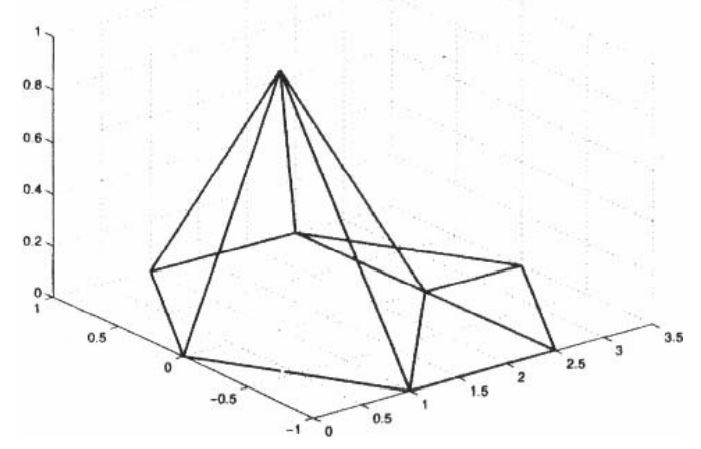
\includegraphics[width=0.6\linewidth]{ch13_7}
	\caption{\textsf{MATLAB's graphical rendition of the basis function $\Phi_4(x,y)$ of Example 13.1. }}
	\label{pfig:ch13_7}
\end{figure}
Given a triangulation of a domain and any function or data / defined on the 
 $N_1, N_2, \cdots, N_m$, the \textbf{finite element interpolan}t of this function/data is given by: 

$$ \sum_{j=1}^{n} f(N_j) \Phi_{N_j}(x,y)$$

We point out that the graph of this interpolant is most easily obtained by simply using the trimesh command directly on the triangle matrix and corresponding values of $f$ ; the calculations for the basis functions are not necessary. This will not be the case for more general elements (see Exercise 26). 
\\

We stress that in the determination of the hat functions $\Phi_j$ , we really split up the problem into determining $\Phi_j$, on each element (triangle). On each element $T_t, \Phi_j(x,y)=a_t^j+b_t^j+c_t^j$ is a linear combination of the three functions $x,y$, and 1. These three functions are a basis for the set of all linear functions on $T_t$.We refer to them as a \textbf{local basis}, to distinguish them from the (global) basis functions $\Phi_j$ . Although these local basis functions are quite natural and have simple formulas, there is another local basis that often has theoretical advantages. To simplify notation, we fix an element $T = T_n$ and denote its three vertices by 
$v_1,v_2$, and $v_3$ (the exact ordering is unimportant, but let's assume they are numbered in counterclockwise order). The corresponding three standard \textbf{local basis functions} $\Phi _1,\Phi_2$, and $\Phi_3$ are the linear functions determined (exactly) by the following conditions: 

\begin{equation}
	\Phi_i(V_j)=\delta_{ij}\equiv 
			\begin{cases}
				1~~~~if~i=j.\\
				0~~~~if~i\neq j.
			\end{cases}
\end{equation}
(The symbol $\delta_{ij}$ is called the \textbf{Kronecker delta symbol}.) It was described earlier how each of these functions can be expressed using the original local basis functions. In terms of these local basis functions, any linear function $\Phi(x,y)$ can be conveniently expressed as:

\begin{equation}
\Phi(x,y)=\Phi(V_1)\Phi(x,y)+\Phi(V_2)+\Phi_2(x,y)+\Phi(V_3)\Phi(x,y)
\end{equation}

(\textit{Proof}: Both sides are linear functions that agree at the three noncollinear points $V_1,v_2$ and $v_3$ and so must be identical.) Each basis function $\Phi$ is simply made up of pieces of corresponding elements containing the node associated with $\Phi$, and each of these pieces is a linear combination (8) of the above local basis functions for its element. The previous example thus gave efficient strategies for computing all of the local basis functions as well as the corresponding basis functions.
\\
\\
EXERCISE FOR THE READER 13.2: (a) Explain why piecewise linear basis 
 could not be used if rectangular elements (with sides parallel to the axes) were used in place of triangular ones. 
\\
(b) Give an example of a simple type of basis function that could be used for such rectangular elements. Make sure that your construction will ensure that anygiven basis function will be continuous across element edges.
\\
\\
As mentioned Section 13.1, triangulation is an art, and as such there has been a notable amount of research in the development of efficient and effective triangulation and mesh generation schemes. One particularly successful and often used method in this area is that of the \textbf{Delaunay triangulation}, relative to a given finite set of points in the plane. This triangulation will result in a set of triangles whose vertices coincide with the given finite set (of nodes) and with the further property that the circumcircle of each triangle in the collection contains only nodes that are vertices ofthat triangle. This condition favors well-rounded triangles over thin ones, which are better for the FEM.
\\
\\
Definitions: Suppose that we have a set of distinct points $P=\left\{ p_1,p_2, \cdots,p_n \right\}$ in the plane $ \mathbb{R}^2$. The Delaunay triangulation relative to $P$ consists of all triangles connecting three noncollinear points $p_i,p_j,p_k \in P$ with the property that there exists a point $a \in \mathbb{R}^2$ which lies equidistant to each of the points $p_i,p_j,p_k$ and closer to these three than to any other point $p_t \in P,\mathfrak{l} \neq i, j k$. 
\\

Figure 13.8 illustrates the Delaunay triangulation for a very small set of four points. It can be shown that the Delaunay triangulation of a finite set of points will always be a triangulation for the \textbf{convex hull}
\footnote{The convex hull of a set of points is the smallest convex set which contains each of the points. There is a degenerate case in which some four of the points lie on a common circle (with no other points inside this circle). Here no three of the points will lie any closer to the center of the circle than the fourth. In algorithms for the Delaunay triangulation what is usually done in degenerate cases is that one of the points is slightly perturbed (moved). Since the area of a circle is zero, the probability that a fourth point will lie on the circle determined by three points is zero. In degenerate cases "the" Delaunay triangulation is not unique. The whole subject of triangulation and more general mesh generation has become quite an important discipline in itself. Good references are Chapter 13 of [Ros-00] and [Ede-01]}of this set. The Delaunay triangulation has the important property that the minimum angle of any of its triangles is as large as possible for any triangulation of the same set of points (see Section 1.2 of [Ede-01]). This makes the Delaunay triangulation very suitable for the FEM. There is a dual notion of the Delaunay triangulation which leads to an equivalent formulation. We give the relevant definitions: 

\begin{figure}[H]
	\centering
	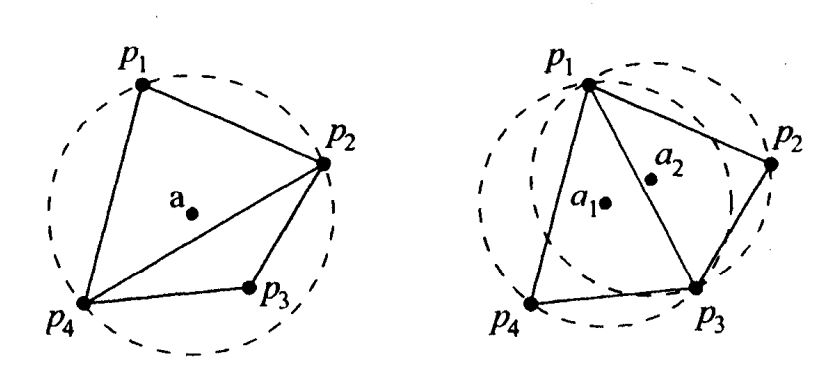
\includegraphics[width=0.6\linewidth]{ch13_8}
	\caption{\textsf{Two triangulations are shown for the same 4-point set $\left\{ p_1,p_2,p_3, p_4 \right\}$. (a) (left) The first one violates the Delaunay condition since $p_3$ lies in the circumcircle of the larger triangle, (b) (right) The second gives the Delaunay triangulation. Circles and centers are drawn in to show the validity of the condition. }}
	\label{pfig:ch13_8}
\end{figure}

\textbf{Definitions}: Suppose that we have a set of distinct points $P=\left\{ p_1,p_2, \cdots,p_n \right\}$ in the plane $\mathbb{R}^2$ (write $p_i=(x_i,y_i))$. Relative to this set, for each $p_i(\leqslant i \leqslant n)$ we define the \textbf{Voronoi region} $V(p_i)$ as: 

\begin{equation}
V(p_i)= \left\{ p \in \mathbb{R}^2 : |p-p_i| \leqslant |p-p_t|~~for~~each~~p_t \in P, \mathfrak{l} \neq i  \right\}
\end{equation}

Here absolute values denote the Euclidean distance (this coincides with the 2-norm introduced in Chapter 7). The \textbf{Voronoi diagram} for P is simply an illustration of the totality of all of the Voronoi regions.
\\

It is not difficult to show that each Voronoi region is a convex set which, if bounded, is a polygon (Exercise 27). In words, the Voronoi region $V(p_i)$ is simply the set of all points in the plane whose closest element of the set $P$ is $p_i$. If a school district wished to minimize bussing times and costs, and if the points /?. represented locations of schools, the Voronoi region of a given school would roughly include all households whose children would be sent to that school. 
\\

The duality result states that two points $p_i, p_j \in P$ are joined by an edge in the Delaunay triangulation if and only if their Voronoi regions $V(p_i)9 V(p_j)$ share a common edge. The Ukrainian mathematician Georges Voronoi was the first to introduce his concept in 1908 [Vor-08]. Subsequently, Russian mathematician Boris Delaunay introduced his triangulation in a 1934 paper [Del-34] that he dedicated to Voronoi. These concepts have numerous applications; details of the rich and interesting history can be found in the book [OkBoSu-92], which contains over 600 references. Construction of the Delaunay triangulation for a given set of points in the plane has been the focus of much research. The first algorithms that were discovered worked in $0(n^4)$ time, but modern refined algorithms perform in$ O(n log n)$ time. Some survey articles of this area are: [SuDr-95] and [BeEp-92], see also Chapter 13 of [Ros-00]. We will make use of MATLAB's built-in functions that will perform both of the Delaunay triangulation and the Voronoi diagrams, so the task of triangulations will thus be reduced to the more simple problem of node deployment. 
\\
We proceed now to introduce the relevant MATLAB functions: 
\\
\\
\begin{center}
\begin{tabular}{|c|l|}
\hline
&If $x$ and $y$ are vectors of the same length n giving the\\
&coordinates of n (noncollinear) points in the plane, this \\
\texttt{tr i = delaunay(x,y) ->}&command will output an $n \times 3$ matrix \texttt{tri} whose rows \\
&contain the indices (rel. to the x and y vectors) of the \\
&triangles in the Delaunay triangulation. \\
\hline
&If $x$ and $y$ are as above, this command will result in a\\
\texttt{voronoi (x,y) ->}&graphic of the Voronoi diagram

for the set of points
\\
&corresponding to x and y \\
\hline
\end{tabular}
\end{center}
\footnote{Actually, the \texttt{voronoi} command will show only the bounded Voronoi regions (i.e., those that have finite areas). There is an easy way to get MATLAB to show all of the regions; see Exercise for the Reader 13.2.}

Once created, the Delaunay triangulation can be used, just like any other triangulation for the FEM. To view the Delaunay triangulation, we could use the above \texttt{trimes} h command. We illustrate by having MATLAB compute both objects for the set of node values that we used for the diagram in Figure 13.5. The following commands result in the plot shown in Figure 13.9(a). 

\begin{lstlisting}[numbers=none,frame=none]
>> N=[ l l;5/ 2 1; 0 0 ; 1 0;5/ 2 0;7/ 2 0; 1 -1;2. 5 -1] ; 
>> x=N(:,1) ; y=N(:,2) ; 
>> tri=delaunay(x,y), trimesh(tri,x,y) 
>> axis(l-l 4.5 -1.5 1.5]), hold on 
>> plot(x,y,'ro')
\end{lstlisting}

\begin{figure}[H]
	\centering
	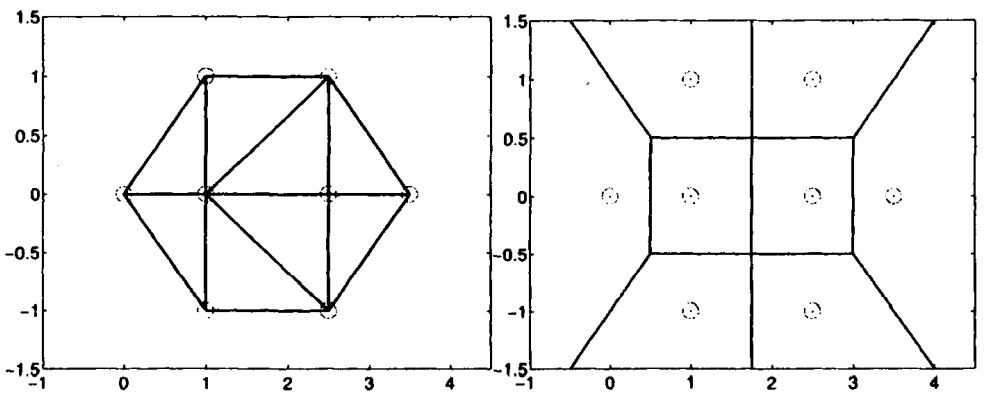
\includegraphics[width=0.6\linewidth]{ch13_9}
	\caption{\textsf{(a) (left) MATLAB plot of the Delaunay triangulation of the set of data points indicated by circles, (b) (right) MATLAB plot of the dual Voronoi diagram for the same set of data points }}
	\label{pfig:ch13_9}
\end{figure}

The Voronoi diagram in Figure 13.9(b) was obtained using the minor modification of the MATLAB's \texttt{voronoi} program that appears in the following exercise for the reader.
\\
\\
EXERCISE FOR THE READER 13.3: (a) Write an M-file called \texttt{voronoial l (x,y )} that will function just like MATLAB's \texttt{voronoi}, except that it will show the unbounded Voronoi regions (not all of them, of course) with a reasonable axis view, (b) Use your program to recreate the plot of Figure 13.9(b).
\\

Some comments are in order. First notice that the Delaunay triangulation that MATLAB gave us coincides with the one we used previously. Also notice that this example demonstrates that the Delaunay triangulation is not unique (so it really should not have been called "the" Delaunay triangulation). Indeed, the two diagonal edges in the center could have been reversed (i.e., reflect the triangulation horizontally) to result in another triangulation that also meets the Delaunay criteria, or the duality theorem's criterion. (The reader should convince himself or herself of these assertions.) The Voronoi regions are of course uniquely defined and so the Voronoi diagram is unique. 
\\

Having the delaunay function to work with makes it a lot easier to do a triangulation; we need only specify the node points. This should be done in a way that will give rise to a Delaunay triangulation whose triangles do not get too thin. A good general rule is to deploy node points in more or less squarelike configurations. The sizes of adjacent squares should not change too abruptly. Of course, when approaching the boundary, special care must be exercised. For boundary value problems, nodes need to be put on the boundary as well. It is also possible to increase the density of nodes in certain parts of the domain in regions where coefficients of the PDE are more active (oscillatory). The next example will create three different triangulations for the same domain, a disk.
\\
\\
\subsubsection{EXAMPLE 13.2:}
Let $\Omega$ denote the unit disk $\left\{ p=(x,y) \in \mathbb{R}^2: \Vert p \Vert_2 \leqslant 1 \right\}$.
\footnote{We are using here the norm notation from Chapter 7: $\Vert p \Vert = \Vert (x,y)\Vert_2\equiv \sqrt{x^2+y^2}$ is in 2-norm which is simply the (planar) Euclidean distance from $p =(x,y)$ to the origin (0,0) . }
Use MATLAB to create and plot three different triangulations of $\Omega$ each having between 1000 and 2000 nodes for each of the three requirements: 
\\
(a) The nodes are more or less uniformly distributed.
\\ 
(b) The density of the nodes increases as $\Vert p\Vert_2$ increases, i.e., as we approach the boundary.
\\ 
(c) The distribution of the nodes increases near the boundary point (1,0). NOTE: We left the exact number of nodes somewhat flexible since we want to stress node deployment schemes and do not wish to be distracted with trying to use a precise number of nodes.
\\
\\
SOLUTION: Part (a): We will give two different strategies for this part. 
\\
\\
\textit{Method I}: We use a squarelike configuration for the nodes. For the most part, 
this will be quite a simple scheme, but near the boundary circle $\Vert p\Vert_2=1$, things get a bit awkward. The square $S=\left\{ p=(x,y) \in \mathbb{R}^2: -1\leqslant x, y\leqslant1 \right\}$includes the disk $\Omega$ as its inscribed circle. Since the ratio of the areas of $\Omega$ to $S$ is $\pi \cdot 1^2 /(2\cdot 2 ) = \pi/ 4 = 0.785\cdots$, it follows that if we uniformly distribute a large number of nodes in the interior of$S$ , roughly $78.5\%$ of them will be in the interior of $\Omega$ . Since it is a simple matter to uniformly distribute any (square) number of nodes in $S$, we will begin by uniformly distributing about 2000 nodes in $S$ , and let $\delta$ denote the square side length that is used. Of these nodes we will keep all of them that lie inside of $\Omega$ but at a distance of at least $\delta/2$ from the boundary circle $\Vert p \Vert_2=1$. Then we add on a set of nodes on the boundary circle, which are uniformly spaced with gaps about equal to $\delta$. The total amount of nodes thus constructed for $\Omega$ will be (well) over 1000 and certainly less than 2000. 
\\
\\
To begin, since $\sqrt{2000} = 44.721...$, we will first construct a square grid of $N_0 = 45^2 = 2025$ interior nodes in $S$ . The horizontal and vertical gaps should be
$\delta = 2/(45 +1)$. The following MATLAB commands will create these nodes, and 
store them in two vectors \texttt{xO, yO} . 

\begin{lstlisting}[numbers=none,frame=none]
>> delta =2/46; counter=l; 
for i=l:45 
for j=l:45 
	xO(counter)=-l+i*delta; yO(counter)=-l+j*delta; 
	counter=counter+l ; 
end 
end 
\end{lstlisting}
Next, from these two vectors we extract those components corresponding to points 
which lie within the slightly smaller circle $\Vert p \Vert_2=1-\delta /2$ the newly created vectors will be labeled as $x$ and $y$. 

\begin{lstlisting}[numbers=none,frame=none]
>> counter=l; 
>> for i=l:2025 
	if norm([xO(i) y0(i)],2) < l-delta/2 
		x(counter)=x0(i); y(counter)=y0(i); 
		counter=counter+l; 
	end 
end 
\end{lstlisting}
Finally, since $2\pi/ \delta = 144.5133...$, we tack onto the existing vectors $x$ and $y$ an additional 145 entries corresponding to 145 equally spaced points on the unit circle $\Vert p \Vert_2 =1$. Figure 13.10(a) shows a plot of this node set. 

\begin{lstlisting}[numbers=none,frame=none]
>> for i=l:145 
	x(i+1597)=cos(2*pi/145*i); y (i + 1597)=sin(2*pi/145*i) ; 
end 
>> plot(x,y,'bo'), axis('equal') 
\end{lstlisting}

\begin{figure}[H]
	\centering
	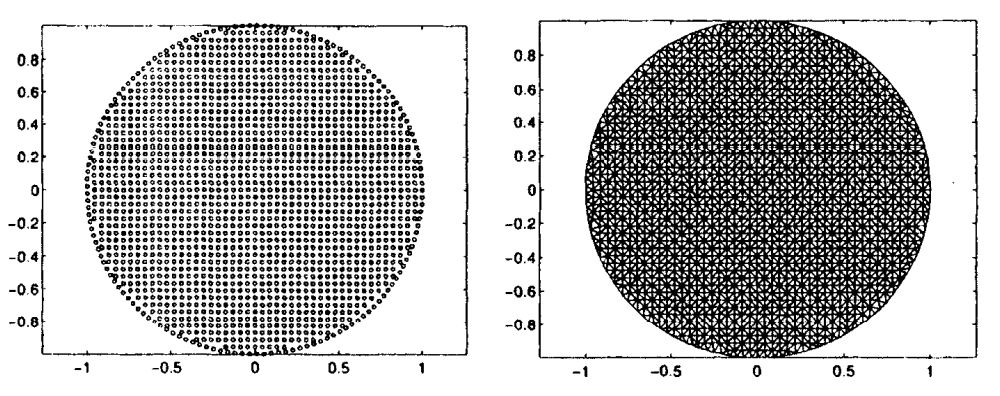
\includegraphics[width=0.6\linewidth]{ch13_10}
	\caption{\textsf{( (a) (left) Grid of nodes from Method 1 of Example 13.2(a), essentially a square pattern except near the boundary. There are 1742 nodes, (b) (right) A corresponding Delaunay triangulation that has 3337 triangles.}}
	\label{pfig:ch13_10}
\end{figure}

The corresponding Delaunay triangulation will result from the following MATLAB commands and is shown in Figure 13.10b. 

\begin{lstlisting}[numbers=none,frame=none]
>> tri=delaunay(x,y); trimesh(tri,x,y), axis('equal')
\end{lstlisting}

\textit{Method 2}: Here we will deploy nodes on circles of increasing radii. The gaps between nodes on a given circle and the gaps between radii of adjacent circles of deployment should be all about equal (uniformity). The final circle will be the boundary of $\Omega$ : $\Vert p \Vert_2 =1$. The only mathematical preliminaries are to decide how many circles to deploy. Letting $\delta$ denote the common gap size, since the radii of the circles increase steadily from 0 to 1, the average radius will be about 1/2, which means the average circumference will be about $2\pi(1/2)=\pi$. Thus the average number of nodes on a circle will be $\pi / \delta$. Likewise, the number of circles of deployment is about MS, so that the total number of nodes will be, roughly, $(\pi/\delta) \cdot (1/\delta)=\pi/\delta^2$. Setting this equal to 1800, say (we want it close to 2000, but to insure the actual number of nodes remains under 2000 we play it a bit safe), and solving for delta gives $\delta = \sqrt{\pi/1800}=0.04177...$ . We may now turn the node deployment over to MATLAB with this scheme: 

\begin{lstlisting}[numbers=none,frame=none]
>> delta=sqrt(pi/1800); x(l)=0; y(l)=0; 
>> nodecount=l; ncirc=floor(1/delta); minrad=l/ncirc; 
>> for i=l:ncirc 
	rad=i*minrad; 
	nnodes=floor(2*pi*rad/delta); 
	anglegap=2*pi/nnodes; 
	for k=l:nnodes 
	  x(nodecount+l)=rad*cos(k*anglegap); 
	  y(nodecount+l)=rad*sin(k*anglegap); 
	  nodecount = nodecount+1; 
	end 
end
\end{lstlisting}

The plotting of the nodes and then the Delaunay triangulation is done just as in 
Method 1 above; the results are shown in Figure 13.11. 

\begin{figure}[H]
	\centering
	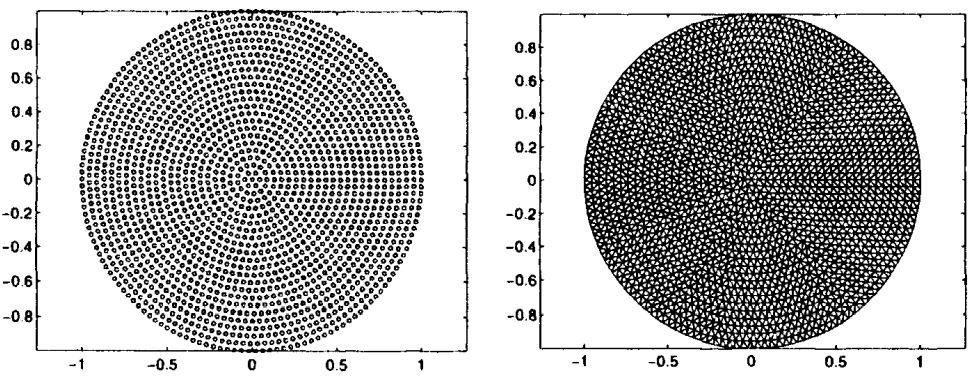
\includegraphics[width=0.6\linewidth]{ch13_11}
	\caption{\textsf{(a) (left) Grid of nodes from Method 2 of Example 13.2(a). There are 1887 nodes, (b) (right) A corresponding Delaunay triangulation that has 3438 triangles. Both the node distribution as well as the Delaunay triangulation take on an aesthetically more appealing pattern than those of Method 1, since this method better respected the symmetry of the domain. }}
	\label{pfig:ch13_11}
\end{figure}

Part (b): The requirement is rather vague. We will use a deployment scheme similar to that of Method 2 in part (a). The new difficulty is that there will need to


be more circles of nodes of larger radii so it will take more work to estimate the total number of nodes. Such an estimate will depend first on how we plan to distribute the radii for the circles of nodes. Here is (but) one scheme. We start off with a single node at the origin (0,0). Then we move to the circle $\Vert p \Vert_2 =1/2=rad(1)=1-1/2$ and deploy 8 (equally spaced) nodes on this circle. Our next circle is $\Vert p \Vert_2 =3/4=rad(2)=1-1/4$ on which we deploy 2-8 = 16 nodes. After this we deploy $2\cdot = 32$ nodes on the circle. We continue this pattern, so that at the wth circle of deployment will be $\Vert p \Vert_2 =1/2=radn1)=1-1/2^n$ on which we will deploy $2^{n+2}$ nodes. This will continue until the number of remaining nodes is still greater than the number of most recently installed nodes (on the last circle of deployment). The final step will be to put all of the remaining nodes on the unit circle $\Vert p \Vert_2 =2$. This plan will create exactly 2000 nodes. Here now is the MATLAB code needed to create such a set of nodes. 

\begin{lstlisting}[numbers=none,frame=none]
>> xb(l)=0; yb(l)=0; rnodes=1999; %remaining nodes 
>> newnodes=8; %nodes to be added on next circle 
>> radcount=l; Icounter for circles 
>> oldnodes=l; %number of nodes already deployed 
>> while newnodes < rnodes/2 
	rad - 1 - 2 A(-radcount); 
	for i=l:newnodes 
	  xb(oldnodes+i)=rad*cos(2*pi*i/newnodes); 
	  yb(oldnodes+i)=rad*sin(2*pi*i/newnodes); 
	end 
	oldnodes=oldnodes + newnodes; %update oldnodes 
	modes = modes - newnodes; %update modes 
	radcount=radcount+l; %update radcount 
	newnodes = 2*newnodes; %update newnodes 
	end 
% now deploy remaining nodes on boundary 
>> for i = l: modes 
	  xb(oldnodes*i)=cos(2*pi*i/rnodes); 
	  yb(oldnodes+i)=sin(2*pi*i/rnodes); 
end
\end{lstlisting}

\begin{figure}[H]
	\centering
	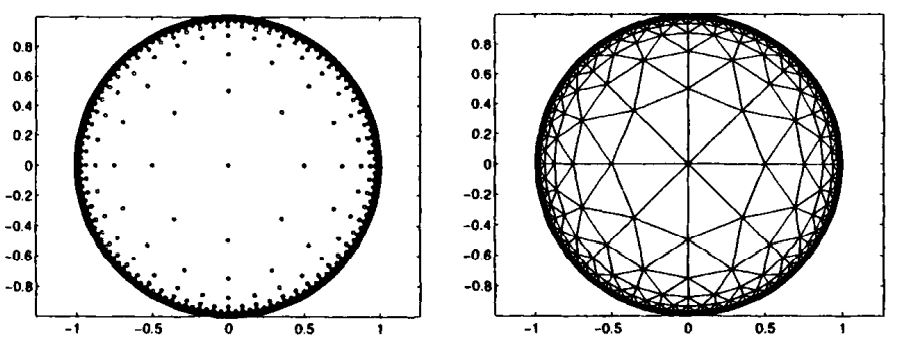
\includegraphics[width=0.8\linewidth]{ch13_12}
	\caption{\textsf{ (a) (left) Grid of nodes for Example 13.2(b). There are 2000 nodes, (b) (right) A corresponding Delaunay triangulation that has 3015 triangles. Such a triangulation is useful for BVPs which are particularly sensitive to boundary data.}}
	\label{pfig:ch13_12}
\end{figure}

The plotting of the nodes and creation of the Delaunay triangulation is obtained in the same fashion as in part (a). The results are shown in Figure 13.12. 
\\
Part (c): The way we will deploy nodes is to first partition $\Omega$ into subsets determined by the regions between pairs of circles centered at (1,0). For each positive integer $n$, we define the following subset $\Omega_n \subseteq \Omega$ : 

$$
\Omega_n= \left\{(x,y) \in \Omega: 1/2^2 < dist((x,y),(1,0)) < 2 \cdot (1/2^n) \right\}
$$

In words, $\Omega_n$ is just the portion of points inside $\Omega$ that lie in between the two concentric circles with center (1,0), and radii $1/2^n$ and $2\cdot(1/2^n)$. A typical such region is illustrated in Figure 13.13. The idea will be to deploy roughly a fixed number of nodes (we will use about 100) in each of these regions, up to a certain value of the index. We will also need to put some nodes in the remaining part of $\Omega$ (which actually can be written as $\Omega_0$); here we again put roughly the same number, about 100 nodes. To decide how to put the nodes on the boundary circle of $\Omega$ as well as in the interior of the domains $\Omega_n$, we use the following estimates. From Figure 13.13, it is clear that $\Omega_n$, is always contained in the half annulus (enclosed between the two dotted circles in the figure), and consequently, 

$$
Area(\Omega)\leqslant \frac{1}{2}[\pi \cdot(2 \cdot2^{-n})^2 -\pi \cdot(2^{-n})^2]=\frac{3\pi}{2}2^{-2n}.
$$

\begin{figure}[H]
	\centering
	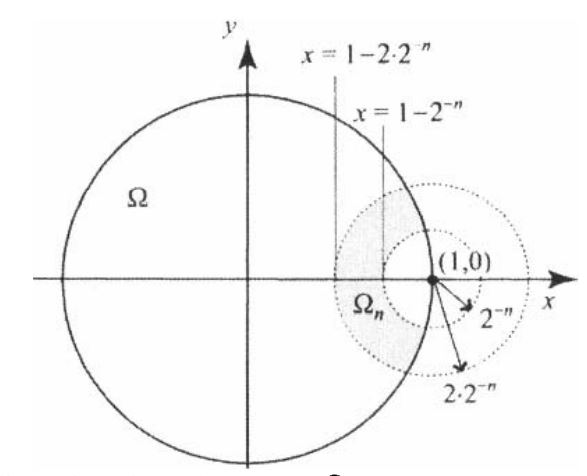
\includegraphics[width=0.6\linewidth]{ch13_13}
	\caption{\textsf{  Illustration of a typical region $\Omega_n$ (shaded) for the triangulation scheme of part (c) of Example 13.2. Such regions are useful for general triangulation schemes when it is desired to have large finer meshes near a special point of the domain. }}
	\label{pfig:ch13_13}
\end{figure}

Also, the estimate becomes increasingly accurate as n gets larger. Now, if we deploy a square grid of nodes with (horizontal = vertical) grid spacing = s in the interior $\Omega_n$, each node would give rise to a square of area $s^2$ inside of $\Omega_n$ (to be specific, let's say that the node gets associated with the square of side length s having the node as its lower left vertex). Thus, if we were to put a grid of 100 such nodes in the interior of $\Omega_n$, the area bound above would yield the following estimate for s:

$$
100 \cdots^2 \leqslant Area(\Omega_n)\leqslant \frac{3\pi}{2}2^{-2n}\Rightarrow s \leqslant \sqrt{3\pi} 2^{-n} /(10\sqrt{2})
$$

We use this as a scheme for the horizontal/vertical grid gap to put between nodes that lie inside each $\Omega_n$. The actual number of nodes on each deployment will be less than 100 because the above estimates are inequalities. Since we will essentially be placing 100 nodes at each iteration on Qw(and the corresponding portion of the boundary circle adjacent to $\Omega_n$ ) starting with $n = 0$, it follows that we should let n run up to about 15 in this scheme. For deploying nodes on the boundary circle that lie adjacent to $\Omega_n$, we also use s as the gap (this time the circular arclength gap) between boundary nodes. Since the boundary circle has radius one, angles are equal to the corresponding boundary arclengths. We will create the nodes using nested loops. On each iteration for $n$ (master loop), the loops will first create and store the corresponding value of s, determined by using an equality in the above inequality for $s$. 
\\

Next, a double loop will be set up that will run through a horizontal and vertical 
grid that will cover the domain $\Omega_n$ and have (horizontal = vertical) grid gap = $s$. 
For this part, note (again from Figure 13.13) that the domain $\Omega_n$ is always 
contained within the rectangle: $R_n = \left\{ (x,y): 1 - 2 \cdot 2^{-n} \leqslant x \leqslant 1, - 2 \cdot 2^{-n} \leqslant y \leqslant2 \cdot 2^{-n} \right\}$ 
Grid points lying in the interior of $\Omega_n$ are added as nodes. Once this 
double nested loop has been executed and interior nodes have been added, the 
same master loop will then move on to install nodes on the two portions of the 
boundary of $\Omega_n$ that lie on the unit circle (= boundary of the main domain $\Omega$ ). 
We will need to compute the angles (made from (0,0) to the positive jc-axis) of the 
two endpoints of the top boundary arc of $\Omega_n$ on the unit circle. (The node 
deployment on the bottom symmetric boundary arc can be gotten by simply 
negating the y-coordinates of the nodes in the upper arc.) It is easily shown using 
the law of cosines that these two angles $\theta_1$ and $\theta_2$ (which technically should be 
denoted by $\theta_{1,n}$ and $\theta_{2,n}$ to indicate their dependence on 
$ \Omega_n$ satisfy: $cos(\theta_n)= 1-2/2^{2n}$
and $cos(\theta_2) = l-2^{-2n}/2$
The following MATLAB code is an 
implementation of the scheme described above. 

\begin{lstlisting}[numbers=none,frame=none]
>> n=0; nodecount-1; 
>> while n<16 
	s=sqrt(3*pi/2)/10/2An; hgrid=2/s/2An; vgrid=4/s/2An; 
%these will be sufficient horizontal and vertical grid counts to 
%create a rectangular grid (with gap size =s) that will cover the 
%domain Omega_n 
	for i=l:hgrid 
	for j=l:vgrid 
	 xnew=1-2/2 A
	 n+ i *s; ynew*-2/2 An+j *s; 
	pij * [xnew ynew]; p=[l 0]; 
 if norm(pij,2)<l-s/2 & norm(pij-p,2)<2/2An & norm(pij-p,2)>l/2An+s/2 
%The three conditions here check to see if the node should be added. 
%The first says that the node should be in the unit circle (with a 
%safe distance to the boundary to prevent interior nodes from getting 
%too close to boundary nodes which will be added later) . The second
%and third state that the distance from the node to the special 
%boundary point (1,0) should be between the two required radii. The 
%last condition has a safety term added to the lower bound to prevent 
%nodes from successive iterations from getting too close. 
	x(nodecount)=xnew; y(nodecount)=ynew; nodecount=nodecount+l; 
  end 
 end 
end 
%The next part of the loop puts nodes on the boundary. 
	thetal=acos(l-2/2A
	(2*n)); theta2=acos(1-2A
	(-2*n)/2); 
	if n==0, thetal*thetal-s; end 
	for theta = thetal:-s:(theta2+s/2) 
  	  x(nodecount)=cos(theta); y(nodecount)=sin(theta); 
	  x(nodecount+l)=cos(theta); y(nodecount+1)=-sin(theta); 
	  nodecount=nodecount+2; 
	end 
	n=n+l; 
end 
%We need to put a node at the special unsymmetric point (-1,0). 
x(nodecount)=-1; y(nodecount)=0; nodecount=nodecount+l; 
%Finally we put nodes in the portion of the domain between (1,0) 
%and the last Omega_n, and then on the boundary. 
%We need first to bump n back down one unit. 
n=n-l; 
 for i=l:hgrid 
 for j=l:vgrid 
	xnew=l-2/2A	n+i*s; ynew=-2/2An+j*s; 
	pij = [xnew ynew]; p=[l 0] ; 
	if norm(pij,2)<l-s/2 & norm(pij-p,2)< l/2A^n 
	 x(nodecount)=xnew; y(nodecount)=ynew; nodecount=nodecount+l; 
	end 
end 
end 
for theta = -theta2:s:theta2 
	x(nodecount)=cos(theta); y(nodecount)=sin(theta); 
	nodecount=nodecount+l; 
end
\end{lstlisting}
Plotting of the nodes as well as the corresponding triangulation is accomplished exactly as it was done in the above two parts. The results are shown in Figures 13.14 and 13.15. 

\begin{figure}[H]
	\centering
	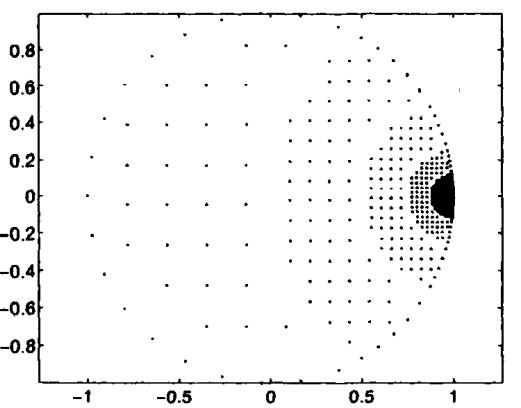
\includegraphics[width=0.5\linewidth]{ch13_14}
	\caption{\textsf{  Node distribution from the solution of part (c) of Example 13.2. The 1457 nodes are constructed in clusters with each cluster getting its grid gap size cut in half as we move in towards the special boundary point (1,0). The exercises will examine some related schemes for this domain where there is a smoother transition in gap sizes of nodes as we progress toward (0,1).  }}
	\label{pfig:ch13_14}
\end{figure}

\begin{figure}[H]
	\centering
	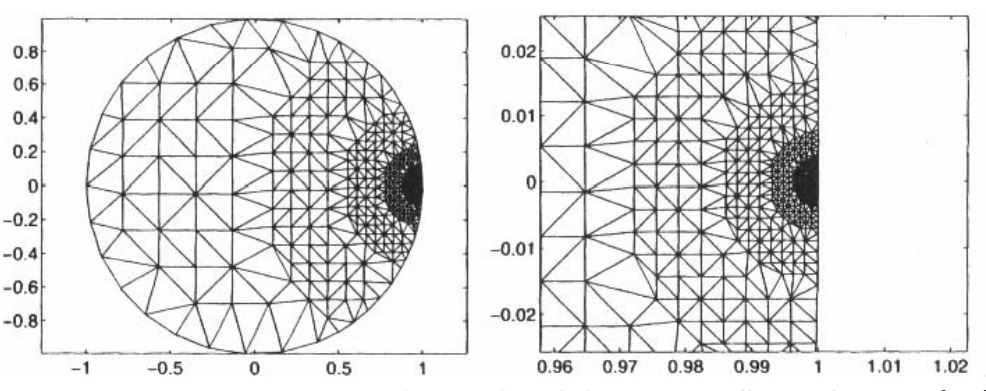
\includegraphics[width=0.8\linewidth]{ch13_15}
	\caption{\textsf{(a) (left) The Delaunay triangulation corresponding to the network of nodes of Figure 13.14 that has 2733 triangles, (b) (right) A $20 \times$ magnification of the triangulation of (a) near the point of focus (1,0).}}
	\label{pfig:ch13_15}
\end{figure}

On the node sets that were constructed in the last example, the Delaunay triangulation worked quite nicely because the domain $\Omega$ was convex. In general, the Delaunay triangulation of a set of nodes will triangulate the convex hull of this set. Delaunay triangulation can still be used to triangulate a nonconvex domain $\Omega$. This is usually done either by breaking up the domain into convex pieces, triangulating each piece, and merging these triangulations or simply by triangulating the convex hull and deleting triangles that are not part of the domain.7 With either strategy, some sort of (global) reindexing will be necessary when constructing the final triangulation. Our next example will illustrate the latter strategy and the exercise for the reader which follows will require also the former strategy. 






















\end{document}